\documentclass[10pt, landscape]{article}
\usepackage[scaled=0.92]{helvet}
\usepackage{calc}
\usepackage{multicol}
\usepackage[a4paper,margin=3mm,landscape]{geometry}
\usepackage{amsmath,amsthm,amsfonts,amssymb}
\usepackage{color,graphicx,overpic}
\usepackage{hyperref}
\usepackage{newtxtext} 
\usepackage{enumitem}
\usepackage[table]{xcolor}
\usepackage{mathtools}
\setlist{nosep}
% for including images
\graphicspath{ {./images/} }

\pdfinfo{
  /Title (CS4225.pdf)
  /Creator (TeX)
  /Producer (pdfTeX 1.40.0)
  /Author (Gavin Chiam)
  /Subject (CS4225)
/Keywords (CS4225, nus,cheatsheet, pdf, notes)}

% Turn off header and footer
\pagestyle{empty}

% redefine section commands to use less space
\makeatletter
\renewcommand{\section}{\@startsection{section}{1}{0mm}%
  {-1ex plus -.5ex minus -.2ex}%
  {0.5ex plus .2ex}%x
{\normalfont\large\bfseries}}
\renewcommand{\subsection}{\@startsection{subsection}{2}{0mm}%
  {-1explus -.5ex minus -.2ex}%
  {0.5ex plus .2ex}%
{\normalfont\normalsize\bfseries}}
\renewcommand{\subsubsection}{\@startsection{subsubsection}{3}{0mm}%
  {-1ex plus -.5ex minus -.2ex}%
  {1ex plus .2ex}%
{\normalfont\small\bfseries}}%
\makeatother

\renewcommand{\familydefault}{\sfdefault}
\renewcommand\rmdefault{\sfdefault}
%  makes nested numbering (e.g. 1.1.1, 1.1.2, etc)
\renewcommand{\labelenumii}{\theenumii}
\renewcommand{\theenumii}{\theenumi.\arabic{enumii}.}
\renewcommand\labelitemii{•}
\renewcommand\labelitemiii{•}

\definecolor{mathblue}{cmyk}{1,.72,0,.38}
\everymath\expandafter{\the\everymath \color{mathblue}}

% Don't print section numbers
\setcounter{secnumdepth}{0}

\setlength{\parindent}{0pt}
\setlength{\parskip}{0pt plus 0.5ex}
%% adjust spacing for all itemize/enumerate
\setlength{\leftmargini}{0.5cm}
\setlength{\leftmarginii}{0.5cm}
\setlist[itemize,1]{leftmargin=2mm,labelindent=1mm,labelsep=1mm}
\setlist[itemize,2]{leftmargin=4mm,labelindent=1mm,labelsep=1mm}
\setlist[itemize,3]{leftmargin=4mm,labelindent=1mm,labelsep=1mm}

% adding my commands
% tightcenter
\newenvironment{tightcenter}{%
  \setlength\topsep{0pt}
  \setlength\parskip{0pt}
  \begin{center}
    }{%
  \end{center}
}

% boxed
\newenvironment{tightbox}{%
  \setlength\topsep{0pt}
  \setlength\parskip{0pt}
  \begin{center}
    \begin{tabular}{|@{\hspace{\dimexpr\fboxsep+0.5\arrayrulewidth}}c@{\hspace{\dimexpr\fboxsep+0.5\arrayrulewidth}}|}
      \hline
    }
    {%
    \\ \hline
    \end{tabular}
  \end{center}
}

% fixed width box
\newenvironment{fixedbox}[1][0.7]{
  \setlength\topsep{0pt}
  \setlength\parskip{0pt}
  \begin{center}
    \begin{tabular}{|>{\centering\arraybackslash}m{#1\linewidth}|}
    \hline
  }{
  \\ \hline
  \end{tabular}
  \end{center}
}

% definition of a new term
\usepackage{soul}
\definecolor{paleyellow}{RGB}{251,243,218}
\newcommand{\definition}[2][]{\sethlcolor{paleyellow}\hl{\textbf{#2}} #1  $\rightarrow$}

% important note (attention)
\newcommand{\attention}{{\color{red}\textbf{! }}}



% -----------------------------------------------------------------------

\begin{document}
\raggedright
\footnotesize
\begin{multicols*}{4}
  % multicol parameters
  \setlength{\columnseprule}{0.25pt}

  \begin{center}
    \fbox{%
      \parbox{0.8\linewidth}{\centering \textcolor{black}{
          {\Large\textbf{CS4225}}
        \\ \normalsize{AY24/25 SEM 1}}
        \\ {\footnotesize \textcolor{gray}{github/Gavino3o}}
      }%
    }
  \end{center}

  \section {Apache Spark}
  \subsection{Hadoop vs Spark}

  \begin{itemize}
    \item \textbf{Hadoop}: Disk-based, MapReduce, HDFS. Not suitable for iterative algorithms as it incurs network and disk I/O overhead for intermediate data.
    \item \textbf{Spark}: In-memory, DAG, RDDs. In the event memory is insufficient, Spark spills data from memory to disk.
  \end{itemize}

  \subsection {Spark Architecture and APIs}
  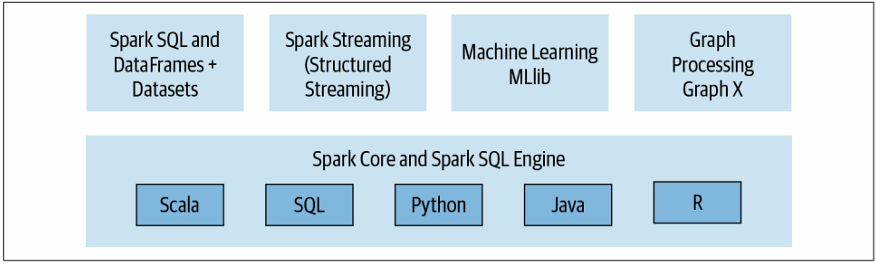
\includegraphics[width=0.95\linewidth]{spark_component_api_stack.png} 
  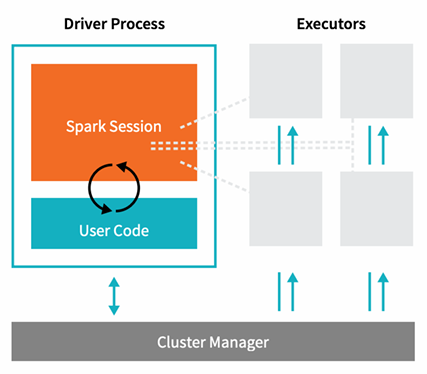
\includegraphics[width=0.95\linewidth]{spark_architecture.png} 
  \begin{itemize}
    \item \textbf{Driver Process}: Manages the execution of the Spark job. Responds to user inputs. Distribute work to the executors.
    \item \textbf{Cluster Manager}: Manages the resources of the cluster. Eg. YARN, Mesos, Kubernetes.
    \item \textbf{Worker Node}: Runs the executors.
    \item \textbf{Executor}: Runs tasks and keeps data in memory or disk storage across them.
    \item \textbf{RDDs}: Resilient Distributed Datasets. A collection of JVM objects. Functional operators (map, filter, etc) are applied to RDDs to transform them.
    \item \textbf{DataFrames}: A distributed collection of data organized into named columns. Similar to a table in a relational database. Expression-based transformation operations. Logical plans and optimisers.
    \item \textbf{Datasets}: A distributed collection of data with a known schema. Combines the benefits of RDDs and DataFrames. Internally rows, externally JVM objects. Typs safe and fast.
  \end{itemize}

  \subsection{RDDs}
  \begin{itemize}
    \item \textbf{Resilient Distributed Datasets}
    \item Fault-tolerant collection of elements that can be operated on in parallel
    \item Immutable, partitioned collection of records
    \item Distributed across a cluster of machines.
  \end{itemize}

  \subsubsection*{Transformations and Actions}
  \begin{itemize}
    \item Transformations are operations that create a new RDD from an existing one.
    \item Lazy evaluation: Transformations are not executed immediately. They are only executed when an action is called. This allows Spark to optimise the execution plan.
    \item Example: \texttt{map}, \texttt{filter}, \texttt{flatMap}, \texttt{groupByKey}, \texttt{reduceByKey}, \texttt{join}, \texttt{order}, \texttt{select}
    \item Actions are operations that return a value to the driver program after running a computation on the dataset.
    \item Example: \texttt{collect}, \texttt{count}, \texttt{reduce}, \texttt{saveAsTextFile}, \texttt{foreach}, \texttt{take}, \texttt{show}
    \item Execution of transformations and actions are executed in parallel accross different worker machines as RDDs are distributed across different worker machines. Results are returned to the driver program in the final step.
    \item Caching: Persisting RDDs in memory across operations. Useful for iterative algorithms.
    \item \texttt{cache()} is a transformation that persists the RDD in memory.
    \item \texttt{persist(options)} is an action that allows for more control over the persistence of the RDD.
    \item \texttt{unpersist()} is an action that removes the RDD from memory.
    \item We should cache RDDs that are used multiple times in the computation or when it is expensive to recompute the RDD.
    \item If we did not cache the RDD, Spark will recompute the RDD each time it is used in an action.
    \item When worker nodes have insufficient memory, Spark may evict LRU RDDs from memory to disk.
  \end{itemize}

  \subsection{Directed Acyclic Graph (DAG)}
  \begin{itemize}
    \item A DAG is a graph with directed edges and no cycles.
    \item In Spark, the DAG is a logical representation of the computation.
    \item Transformations construct the DAG; actions execute the DAG.
    \item Spark optimises the DAG by combining operations and minimising data shuffling.
    \item Narrow dependencies: Each partition of the parent RDD is used by at most one partition of the child RDD. Example: \texttt{map}, \texttt{filter}, \texttt{flatMap}, \texttt{contains}
    \item Wide dependencies: Each partition of the parent RDD may be used by multiple partitions of the child RDD. Example: \texttt{groupByKey}, \texttt{join}, \texttt{reduceByKey}, \texttt{sortByKey}, \texttt{orderByKey} 
    \item In the DAG, consecutive narrow transformations are combined into a single stage and executed on the same machines. Wide transformations are separated into different stages.
    \item Across stages, data is shuffled across the network, which involves writing intermediate data to disk.
    \item Spark tries to minimise the number of stages and the amount of data shuffled.
    \item \textbf{Lineage}: The sequence of transformations that lead to an RDD.
    \item If a worker node fails, Spark can recompute the lost partitions of an RDD using the lineage. Note: we only need to recompute the lost partitions, not the entire RDD.
  \end{itemize}

  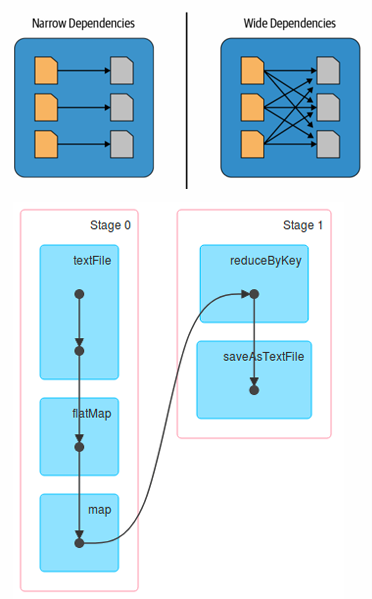
\includegraphics[width=0.95\linewidth, height=185px]{spark_dependency_stages.png}

  \subsection{DataFrames}
  \begin{itemize}
    \item A distributed collection of data organised into named columns.
    \item Similar to a table in a relational database.
    \item Easier to use than RDDs as it has a higher-level API.
    \item All Dataframe operations are still ultimately compiled down to RDD operation by Spark.
    \item Generally, transformation functions take in either strings or column objects.
    \item Transformations are still lazyly evaluated.
  \end{itemize}

  \subsection{Spark SQL}

  \begin{itemize}
    \item Spark SQL is a module for working with structured data.
    \item It provides a programming abstraction called DataFrames and can also act as a distributed SQL query engine.
    \item Spark SQL provides a domain-specific language for working with structured data.
    \item It allows running SQL queries on existing RDDs and DataFrames.
    \item Catalyst optimiser is the Spark SQL query optimiser. It takes a computational query and converts it into an optimised logical plan. Four Phases: Analysis, Logical Optimisation, Physical Planning, Code Generation (Project Tungsten).
    \item Multiple physical plans can be generated for a single logical plan. The optimiser chooses the best physical plan based on cost estimation.
    \item Project Tungsten is the Spark SQL execution engine. It aims to improve performance by optimising memory usage and CPU utilisation.
    \item Tungsten optimises memory usage by using binary processing, cache-aware computation, and code generation.
    \item \textbf{Unified API}: Spark SQL can be used with Java, Scala, Python, SQL, and R. It has one engine for all types of data processing.
  \end{itemize}

  \subsection{Machine Learning with Spark}

  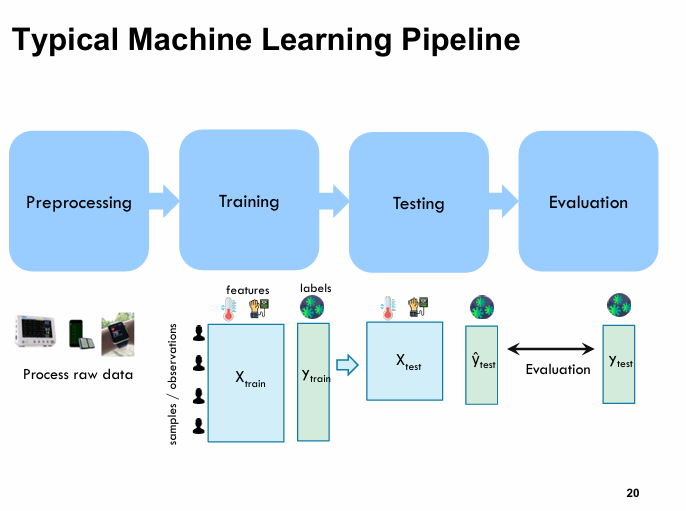
\includegraphics[width=0.95\linewidth]{ml_pipeline.png} 

  \begin{itemize}
    \item Data Quality: Missing values (impute, drop, add column indicating it is missing or not)
    \item Categorical Encoding: Convert categorical variables to numerical variables. Numerical values are often assigned in a way that represents the ordinal relationship between the categories or inherent order among the categories.
    \item One Hot Encoding: Convert categorical variables to binary vectors. Each category is represented by a binary vector. Useful when there is no ordinal relationship between the categories, and to ensure that the categorical variable does not imply any numerical relationship.
    \item Normalization: Scale the features to a standard range. Useful for algorithms that are sensitive to the scale of the input features. Example: clipping, log transform, standard scalerm, min-max scaler.
    \item Logistic Regression: A linear model for binary classification. It models the probability that the output is 1 given the input features. Ultilses the sigmoid function. $\sigma(x) = \frac{1}{1 + e^{-x}}$
    \item $ \hat{y} = \sigma(x \cdot w + b) $
    \item Cross Entroypy Loss: Measures the difference between two probability distributions. It is used as the loss function for logistic regression. $L(y, \hat{y}) = -y \log(\hat{y}) - (1 - y) \log(1 - \hat{y})$
    \item Gradient Descent: An optimisation algorithm that minimises the loss function. It iteratively updates the weights and biases in the direction of the negative gradient of the loss function.
    \item $w_{t+1} = w_t - \alpha \nabla_w L(w_t)$
    \item Evaluation Metrics: Accuracy, Precision, Recall, F1 Score, ROC Curve, AUC.
    \item Accuracy: $\frac{TP + TN}{TP + TN + FP + FN}$
    \item Precision: $\frac{TP}{TP + FP}$
    \item Recall: $\frac{TP}{TP + FN}$
    \item F1 Score: $2 \times \frac{Precision \times Recall}{Precision + Recall}$
    \item Errors: Mean Squared Error, Mean Absolute Error, Root Mean Squared Error.
    \item Mean Squared Error: $\frac{1}{n} \sum_{i=1}^{n} (y_i - \hat{y_i})^2$
    \item Mean Absolute Error: $\frac{1}{n} \sum_{i=1}^{n} |y_i - \hat{y_i}|$
    \item Root Mean Squared Error: $\sqrt{\frac{1}{n} \sum_{i=1}^{n} (y_i - \hat{y_i})^2}$
    \item R Squared Value (0 to 1): Measures the proportion of the variance in the dependent variable that is predictable from the independent variable. The higher the better.
  \end{itemize}

  \subsubsection*{Pipelines}
  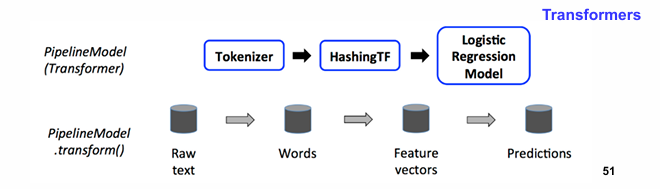
\includegraphics[width=0.95\linewidth]{pipeline_model.png} 
  \begin{itemize}
    \item Benefits: Better code reuse, Easier to perform cross validation, Easier to tune hyperparameters, Easier to productionise the model.
    \item Transformers are the building blocks of a pipeline.
    \item A transformer has a transform() method that takes in a DataFrame and returns a new DataFrame.
    \item Example: VectorAssembler, StringIndexer, OneHotEncoder, StandardScaler, LogisticRegression
    \item Generally, these transformers output a new DataFrame which append their result to the original DataFrame. 
    \item A fitted model (e.g LogisticRegressionModel) is also a transformer. It transforms Dataframe by adding a prediction column.
    \item Estimators is an algorithm that takes in data, and outputs a fitted model. Example: A learnign algorithm like LogisticRegression can be fit to data, producing the trained logistic regression model.
    \item Estimators have a \texttt{fit()} method that takes in a DataFrame and returns a Transformer.
          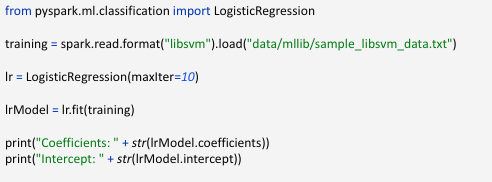
\includegraphics[width=0.95\linewidth]{estimator.png} 
    \item Pipelines are a sequence of stages. Each stage is either a Transformer or an Estimator.
    \item Pipeline itself is an Estimator. It has a \texttt{fit()} method that takes in a DataFrame and returns a PipelineModel.
    \item When \texttt{fit()} is called on a Pipeline, the stages are executed in order. For Transformers, the \texttt{transform()} method is called. For Estimators, the \texttt{fit()} method is called.
    \item The output of \texttt{Pipeline.fii()} is a PipelineModel, which is a Transformer, and consists of a series of Transformers.
    \item The \texttt{transform()} method of the PipelineModel applies the fitted model to the input DataFrame.
  \end{itemize}

  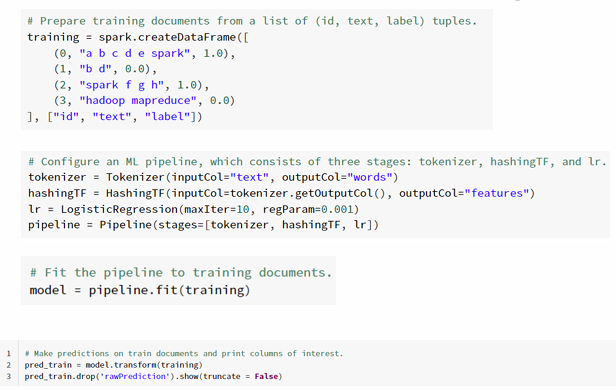
\includegraphics[width=0.95\linewidth]{ml_code_ex1.png}
  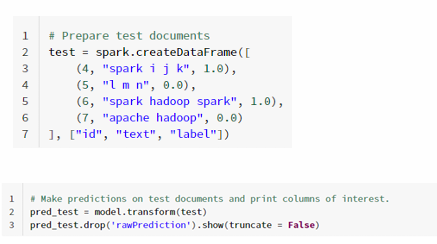
\includegraphics[width=0.95\linewidth]{ml_code_ex2.png} 
  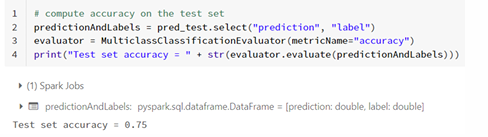
\includegraphics[width=0.95\linewidth]{ml_code_ex3.png} 

  \section{Stream Processing}
  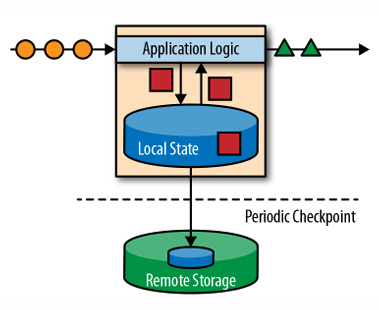
\includegraphics[width=0.95\linewidth]{stream_process.png}
  Goal: Process data in real-time as it is generated. State can be stored and accessed in many different places including program variables, local files, or embedded/external databases.

  \subsection{Micro-Batch Stream Processing}
  \begin{itemize}
    \item Spark Structured Streaming uses a micro-batch processing model.
    \item Data from the input stream is divided into micro batches, each of which will be processed in the Spark cluster in a distributed manner.
    \item Small deterministic tasks generate the output of each micro-batch. Time is divided into small intervals, and data is processed in each interval.
    \item Advantages: quick; recover from failures efficently; deterministic nature ensures end-to-end exactly-once processing.
    \item Disadvantages: latency (cannot handle millisecond); micro-batch size affects latency and throughput; micro-batch processing can be less efficient than true stream processing.
    \item It is sufficient for most use cases.
    \item In Spark Structured Streaming, the input data is treated as an unbounded table. 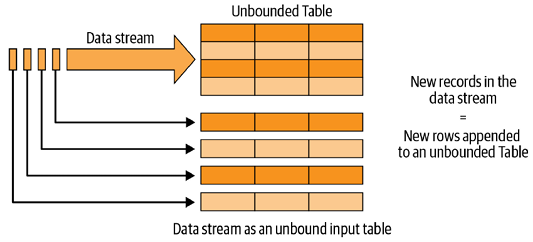
\includegraphics[width=0.95\linewidth]{spark_stream_unbound_table.png}
    \item Five Steps to Define Steaming Query: 
          \begin{enumerate}
            \item Define the input source.
            \item Transform Data.
            \item Define output sink and output mode.
            \item Specifying processing details. (Triggering details, checkpointing, etc)
            \item Start the query.
          \end{enumerate}
  \end{itemize}

  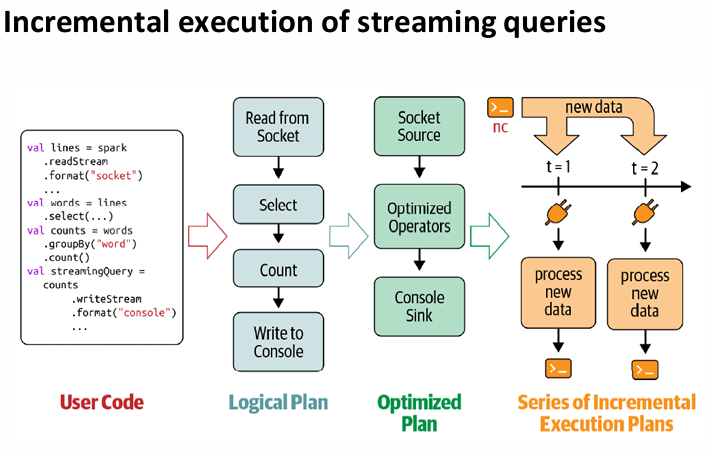
\includegraphics[width=0.95\linewidth]{incremental_excution_stream.png}
  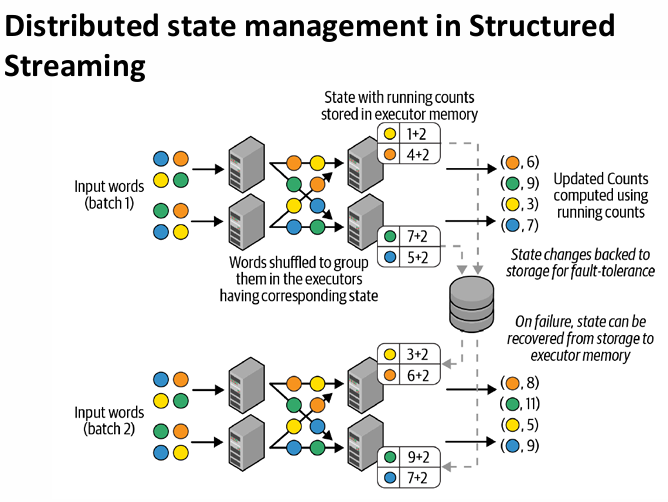
\includegraphics[width=0.95\linewidth]{spark_stream_fault_tolerance.png}

  \subsubsection{Data Transformation}
  \begin{itemize}
    \item \textbf{Stateless Transformations:}
        \begin{itemize}
          \item Process each row individually without needing information from previous rows
          \item Projection operations: \texttt{select()}, \texttt{explode}, \texttt{map()}, \texttt{flatMap()}
          \item Selection operations: \texttt{filter()}, \texttt{where()}
        \end{itemize}
    \item \textbf{Stateful Transformations:}
          \begin{itemize}
            \item Process each row based on information from previous rows.
            \item Example: \texttt{DataFrame.groupBy().count()}
            \item In every micro-batch, the incremental plan adds the count of new 
            records to the previous count generated by the previous micro-batch
            \item The state is maintained in the memory of the Spark executors and is 
            checkpointed to the configured location to tolerate failures.
          \end{itemize}
    \item \textbf{Stateful Streaming Aggregations:}
          \begin{itemize}
            \item \textbf{Aggregations not based on time windows:}
            \begin{itemize}
              \item Global aggregations: \texttt{groupBy().count()}
              \item Grouped aggregations: \texttt{groupBy("sensorId").mean("value")}
              \item Supported aggregations: \texttt{count()}, \texttt{sum()}, \texttt{avg()}, \texttt{min()}, \texttt{max()}, \texttt{countDistinct()}, \texttt{collect\_set()}, \texttt{approx\_count\_distinct()}
            \end{itemize}
            
            \item Processing Time: The time at which the data is processed by the system. (Not deterministic, susceptible to system delays)
            \item Event Time: The time at which the event occurred in the real world. (Deterministic)
            \item Event time decouples the processing speeed from the results. An event time window computation will yield the same result regardless of the processing time.
            \item Watermark: A threshold that determines how late the data can be in event time. Data that arrives later than the watermark is considered late data.
            
            \item \textbf{Aggregations with Event-Time Windows:}
                \begin{itemize}
                  \item Example: \texttt{sensorReadings.groupBy("sensorId", window("eventTime", windowLength, shiftAmt)).count()}
                  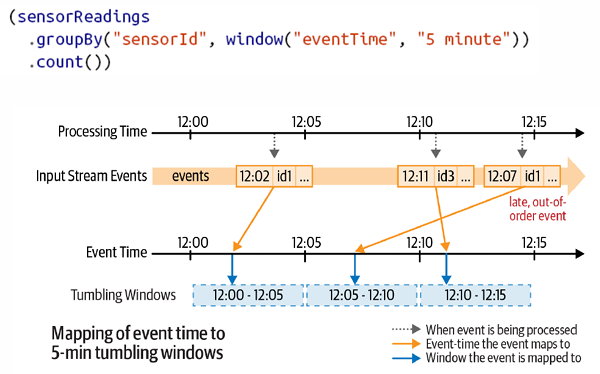
\includegraphics[width=0.95\linewidth]{event_time_no_overlap.png}
                  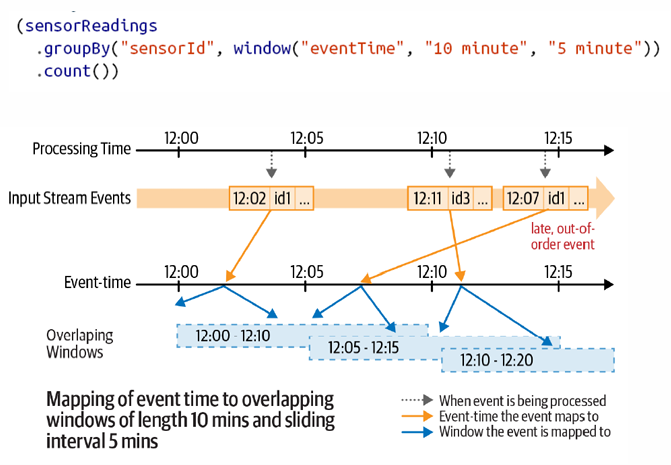
\includegraphics[width=0.95\linewidth]{event_time_overlap.png}
                  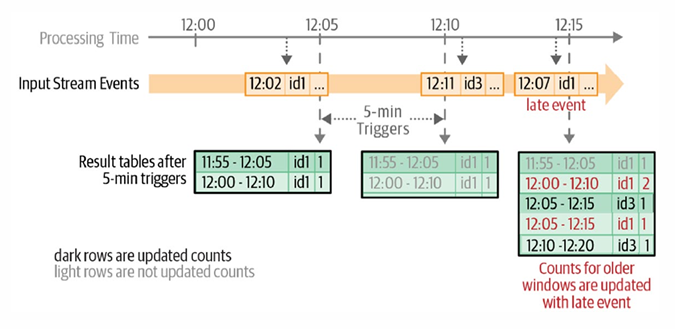
\includegraphics[width=0.95\linewidth]{spark_stream_no_watermark.png}
                  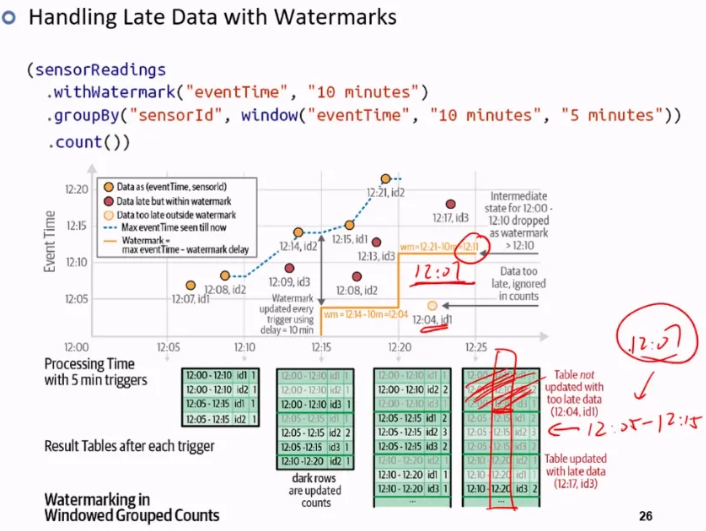
\includegraphics[width=0.95\linewidth]{spark_stream_watermark.png}
                  \item Take the latest \textbf{event time} and minus the watermark time. Let go of the rows in the result window with end interval time lower than calculated time.
                  \item Watermark just determines which window records in the table to drop off. If it was not dropped, it may still be updated even though the late data event time is before the watermark time.
                  \item Data with event time of 12:07 is still updated as the event window 
                  [12:05 $-$ 12:15] is not dropped as the window end interval time is not before the watermark time.
                  \item \textbf{Performance Tuning: }
                      \begin{itemize}
                        \item Cluster resource provisioning appropriately to run 24/7
                        \item Number of partitions for shuffles to be set much lower than batch queries
                        \item Setting source rate limits for stability
                        \item Multiple streaming queries in the same Spark application
                        \item Tuning Spark SQL Engine
                      \end{itemize} 
                \end{itemize}
          \end{itemize}
  \end{itemize}

  \subsection{Flink}
  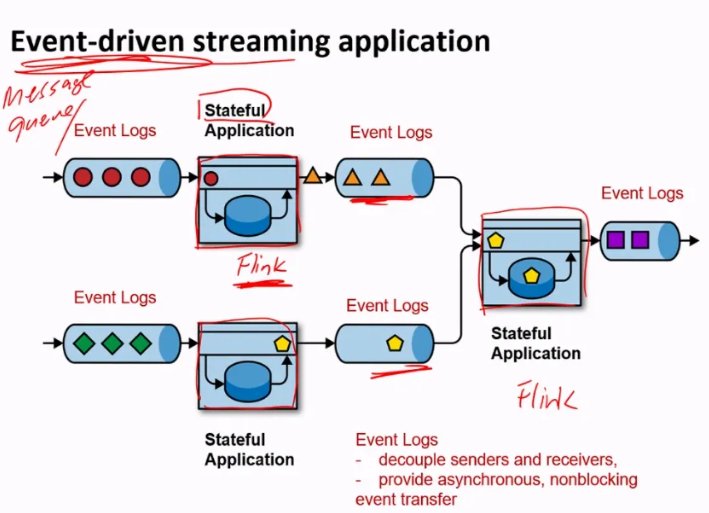
\includegraphics[width=0.95\linewidth]{event_driven_streaming.png}
  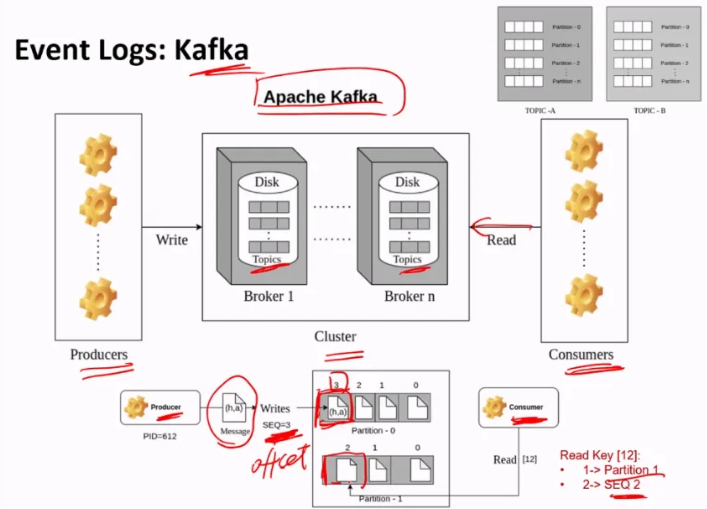
\includegraphics[width=0.95\linewidth]{event_logs_kafka.png}
  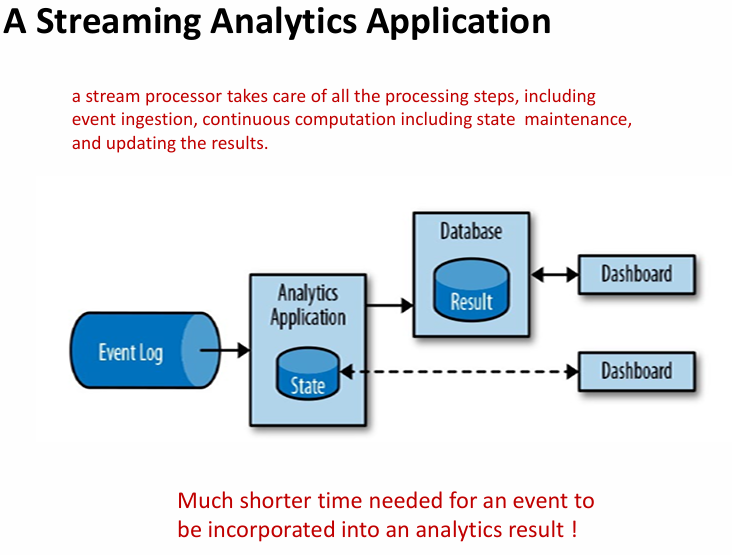
\includegraphics[width=0.95\linewidth]{streaming_analytics_application.png}
  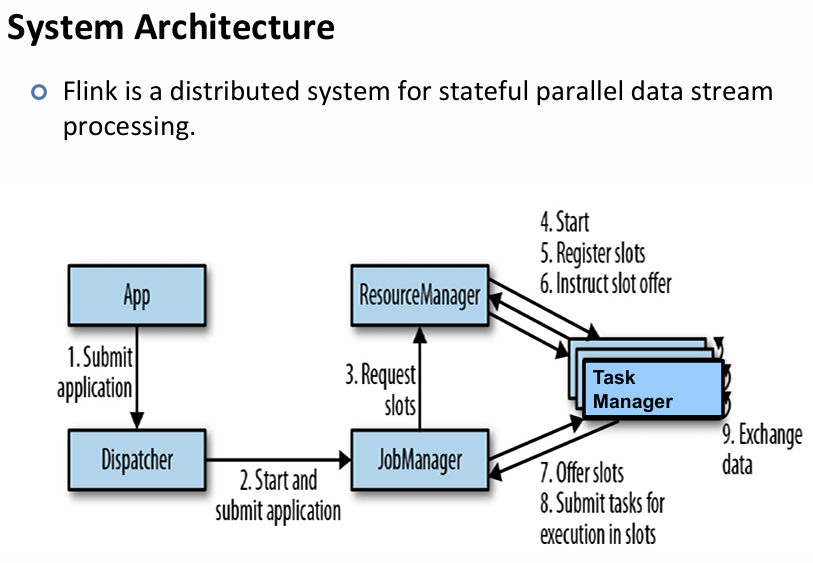
\includegraphics[width=0.95\linewidth]{flink_sys_architecture.png}

  \subsubsection*{Task Execution}
  \begin{itemize}
    \item A Task Manager can run multiple tasks concurrently
          \begin{itemize}
            \item Tasks of the same operator (data parallelism)
            \item Tasks of different operators (task parallelism)
            \item Tasks of different applications (job parallelism)
          \end{itemize}
    \item Task Managers offers certain number of processing slots to control the number of tasks it is able to concurrently execute. Think of slots as CPU cores.
    \item A processing slot can execute one slice of an application, i.e one parallel task of each operator of the application
    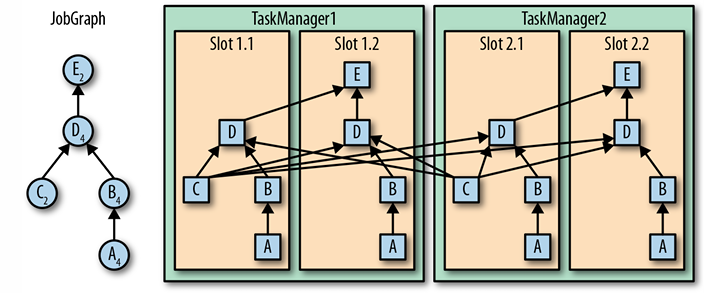
\includegraphics[width=0.95\linewidth]{flink_task_manager.png}
    \item The tasks of a running application are continuously exchanging data.
    \item Task Managers take care of shipping data from sending tasks to receiving tasks.
    \item The network component of a Task Manager collects records in buffers before they are shipped.
    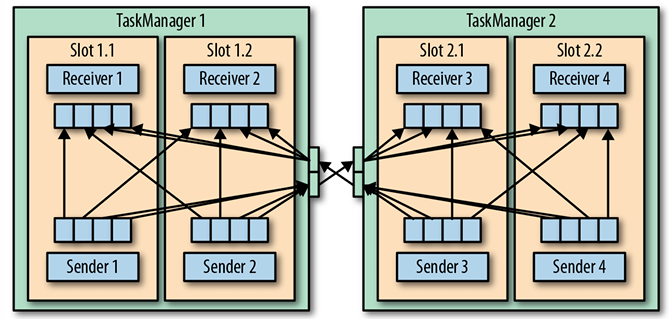
\includegraphics[width=0.95\linewidth]{flink_network_component.png}
  \end{itemize}
  
\subsection{Event-Time Processing in Flink}
\begin{itemize}
  \item Flink allows for event-time processing by allowing the user to assign \textbf{timestamps} to events/records.
  \item Flink can handle out-of-order events by using watermarks.
  \item \textbf{Watermarks} are used to derive the current event time at each task in an event-time application.
  \item In Flink, watermarks are implemented as special records holding a timestamp as a Long value. Wtermarks flow in a stream of regular records with annotated timestamps.
  \item Watermarks in Flink is not directly invovled in late data handling. It is used to determine when to emit results of windowed operations.
\end{itemize}

\subsubsection{Statem Management}

\begin{itemize}
  \item Stateful Stream Processing Task: All data maintained by a task and used to compute the results of a function belong to the state of the task.
  \item \textbf{State Backend:}
       \begin{itemize}
        \item Local State Management: A task of a stateful operator reads and updates its state for each incoming record.
        \item Each parallel task locally maintains its state in memory to ensure fast state accesses.
       \end{itemize}
  \item \textbf{Checkpointing:}
        \begin{itemize}
          \item A Task Manager process may fail at any point, hence its storage must be considered volatile
          \item Checkpointing the state of a task to a remote and persistent storage
          \item The remote storage for checkpointing could be a distributed filesystem or a database system
          \item \textit{Consistent Checkpoints} (similar to Spark's micro-batch checkpointing, Stop the world, not used by Flink)
            \begin{enumerate}
              \item Pause the ingestion of all input streams
              \item Wait for all in-flight data to be completely processed, meaning all tasks have processed all their input data
              \item Take a checkpoint by copying the state of each task to a remote, 
              persistent storage. The checkpoint is complete when all tasks have 
              finished their copies.
              \item Resume the ingestion of all streams.
            \end{enumerate}
          \item To execute failure recovery from consistent checkpointing. Simply restart the application, reset the state of all staetful tasks to latest checkpoint, and resume tasks.
          \item \textbf{Flink Checkpointing Algorithm}
              \begin{itemize}
                \item Chandy-Lamport Algorithm: A distributed algorithm for recording a consistent global snapshot of a distributed system.
                \item Does not pause the application but decouples checkpointing from processing
                \item Some tasks contninue processing while others persist their state
                \item Uses \textbf{checkpoint barrier}, a special record that signals the tasks to persist their state
                \item Checkpoint barriers are injected by source operators into the regular 
                stream of records and cannot overtake or be passed by other records
                \item A checkpoint barrier carries a checkpoint ID to identify the checkpoint it 
                belongs to and logically splits a stream into two parts
                \item All state modifications due to records that precede a barrier are 
                included in the barrier’s checkpoint and all modifications due to records 
                that follow the barrier are included in a later checkpoint.
                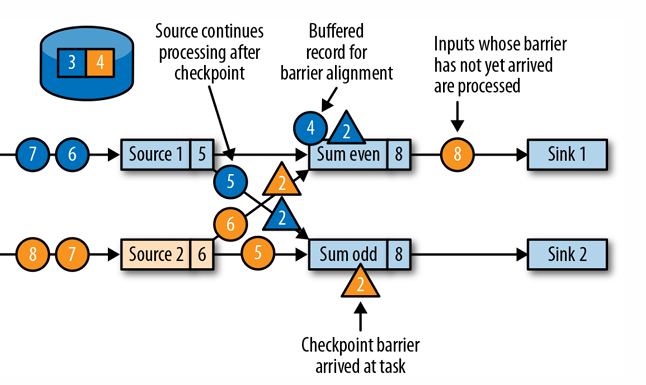
\includegraphics[width=0.95\linewidth]{flink_checkpoint_buffer.png}
                \item Job manager initiates checkpoints by sending message to all sources.
                \item Sources checkpoint their state and emit a checkpoint barrier.
                \item Records from input streams for which a barrier already arrived are buffered.
                \item All other records are regularly processed
                \item Tasks checkpoint their state once all barriers have been received, then they forward the checkpoint barrier
                \item Tasks continue regular processing after the checkpoint barrier is forwarded
                \item Sinks acknowledge the reception of a checkpoint barrier to the JobManager
                \item A checkpoint is complete when all tasks have acknowledged the successful checkpointing of their state
                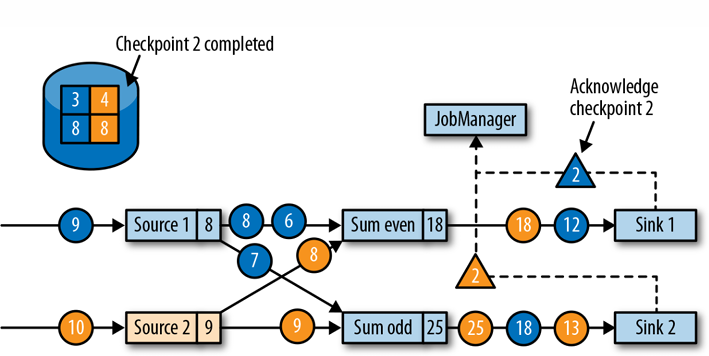
\includegraphics[width=0.95\linewidth]{flink_checkpoint_end_acknowledgement.png}
                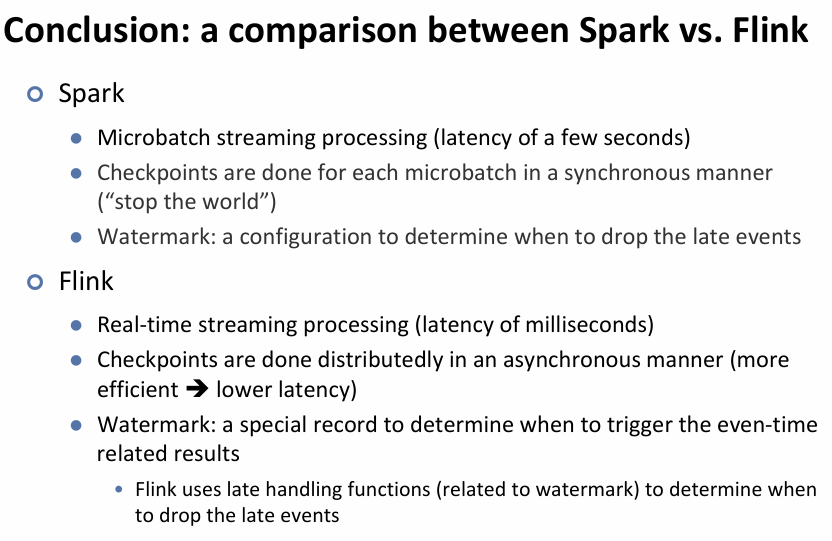
\includegraphics[width=0.95\linewidth]{flink_vs_spark.png}
              \end{itemize}
        \end{itemize}
\end{itemize}

\section{Graphs}

\subsection{Graph Processing}
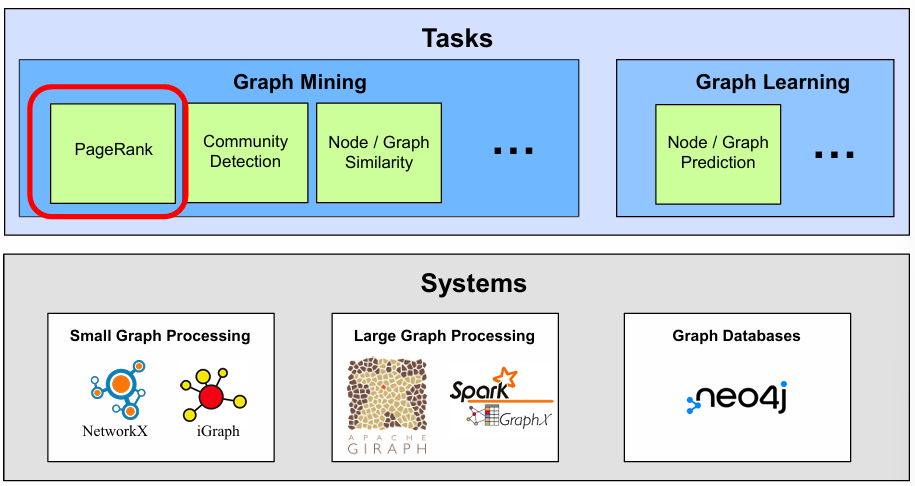
\includegraphics[width=0.95\linewidth]{graph_processing_tech.png}

\subsubsection{Simple PageRank}

\begin{itemize}
  \item We can visualise the web as a directed graph where each page is a node and each hyperlink is an edge.
  \item PageRank is an algorithm that measures the importance of a page in a network.
  \item The importance of a page is determined by the number of incoming links and the importance of the pages that link to it.
  \item If we assume incoming links are harder to manipulate, we can rank each page based on the number of incoming links.
  \item Problem: Malicious users can create a large number of pages that link to a target page to increase its rank.
  \item Solution: Make the rank of a page dependent on the rank of the pages that link to it.
  \item Therefore, links from important pages count more, this is true recursively.
  \item PageRank recursively computes the rank of a page based on the ranks of the pages that link to it. [Weighted edges]
  \item \textbf{Voting Formulation:}
        \begin{itemize}
          \item For each page $j$, we define its importance as $r_j$
          \item If page $j$ with importance $r_j$ has $n$ outgoing links, each link gets $\frac{r_j}{n}$ importance.
          \item Page $j$'s own importance is the sum of the votes on its incoming links.
          \item Formally: $r_j = \underset{i \rightarrow j}{\sum} \frac{r_i}{d_i}$. \newline Where $d_i$ is the number of outgoing links from page $i$.
          \item The sum of importances of pages linking to j, each divided by number of outgoing links from that page.
          \item In the event that the flow equations have no unique solution, we can add an additional constain to force uniqueness:\newline
                $r_a + r_b + r_c = 1$
        \end{itemize}
    \item \textbf{Matrix Formulation:}
          \begin{itemize}
            \item Stochastic adjacency matrix, $M$
            \item Let page $i$ has $d_i$, out-links.
            \item If $ i \rightarrow j $, then $M_{ji} = \frac{1}{d_i} $, else $M_{ji} = 0$
            \item $M$ is a column-stochastic matrix, whjen each column sums to 1.
            \item Let \textbf{Rank Vector} $= r$ and $r_i$ is the rank of page $i$.
            \item $\sum_i r_i = 1$
            \item The flow equation can be written as $r = M \cdot r$
            \item Column points to row. Each column is a page, each row is a page.
            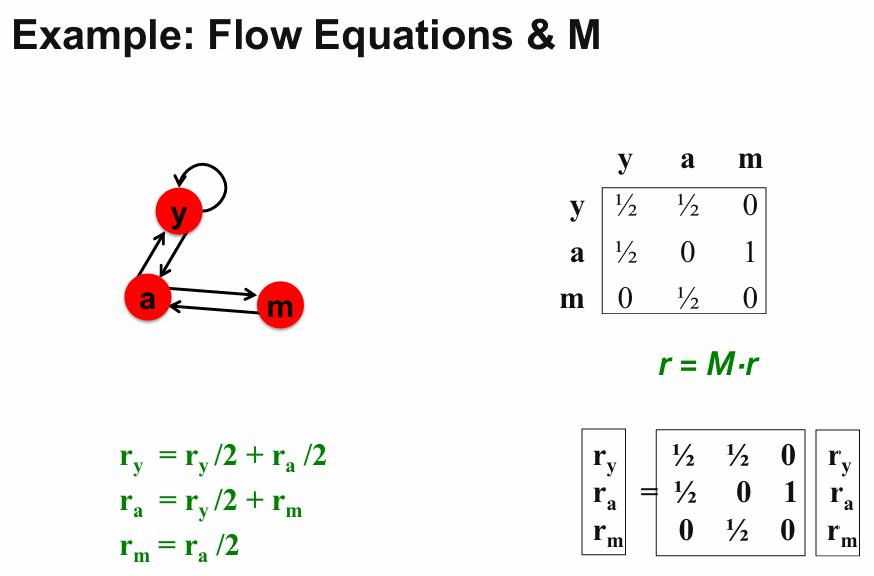
\includegraphics[width=0.95\linewidth]{flow_equation_matrix_example.png}
          \end{itemize}
    \item \textbf{Power Iteration Method:}
        \begin{itemize}
          \item  Each node starts with 
          equal importance (of $\frac{1}{N}$). During each step, each node passes its 
          current importance along its outgoing edges, to its neighbors.
          \begin{enumerate}
            \item Suppose there are $N$ web pages
            \item Initialise: $r^{(0)} = [\frac{1}{N}, ... ,\frac{1}{N}]^T$
            \item Iterate: $r^{t+1} = M \cdot r^{(t)}$
            \item Stop when $ | r^{t+1} - r^{t} |_1 < \epsilon $
          \end{enumerate}
        \end{itemize}
    \item \textbf{Random Walk Interpretation:}
          \includegraphics*[width=0.95\linewidth]{random_walk_interpretation.png}
    \item \begin{itemize}
      \item Stationary Distribution: as $ t \rightarrow \inf $, the probability distribution approaches a steady state, representing the long term probability that the random walker is at each node, which is the PageRank scores.
      \item Three Questions:
          \begin{enumerate}
            \item Does the random walk converge? Not always
            \item Does it converge to what we want? 
            \item Are results reasonable?
          \end{enumerate}
        \item Some pages are \textbf{Dead Ends}: Pages with no outgoing links. Causes importance to leak out of the network. \includegraphics*[width=0.95\linewidth]{deadend.png}
        \item \textbf{Spider Traps}: Pages that link to each other but have no outgoing links. Eventually, all importance will be trapped in the spider trap. \includegraphics*[width=0.95\linewidth]{spider_trap.png}
        \item To solve deadends and spider traps, we cam introduce teleportation. At each step, the random walker has a small probability of teleporting to a random page. This ensures that the random walker can escape deadends and spider traps.
        \item PageRank Equation: $r_j = \underset{i \rightarrow j}{\sum} \beta \frac{r_i}{d_i} + (1 - \beta) \frac{1}{N}$
        \item $\beta$ is also known as the damping factor. It is the probability that the random walker follows a link, and $1 - \beta$ is the probability that the random walker teleports.
        \item Google Matrix A: $A  = \beta M + (1 - \beta) [\frac{1}{N}]_{N \times N} $
        \item PagreRank Equation (Matrix Form): $r = A \cdot r$
        \item In practice, $\beta$ is usually set to 0.8 to 0.9. Which allows for 5 to 10 steps on average before teleport.
        \item If at a Dead End, Always Teleport: preprocess random walk matrix $M$ and set each entry in the column of the dead-end page to $\frac{1}{N}$. This makes the matrix column stochastic. \includegraphics*[width=0.95\linewidth]{teleport_deadend.png}
      
    \end{itemize}
    \end{itemize}
    \subsubsection*{Topic Specific PageRank}
    
    Problems with Simple Page Rank:
    \begin{itemize}
      \item Measures generic popularity of a page and does not consider popularity based on specific topics. Solution: Topic-Specific PageRank.
      \item Uses a single measure of importance. Solution: Hubs-and-Authorities.
      \item Susceptible to link spamming. Solution: TrustRank.
    \end{itemize}

    \begin{itemize}
      \item Idea: Bias the random walk towards a specific topic.
      \item When random walker teleports, it picks a page from a set $S$.
      \item $S$ contains only pages that are relevant to the topicFor each teleport set $S$, we get a different PageRank vector $r_s$.
      \item \begin{equation*}
        A_{ij} =
        \begin{cases}
          \beta M_{ij} + (1 - \beta) \cdot \frac{1}{|S|} &\text{if } i \in S\\
          \beta M_{ij} + 0  &\text{otherwise}
        \end{cases}
      \end{equation*}
       \item $A$ is stoaachstic and column-normalised.
       \item \includegraphics*[width=0.95\linewidth]{topic_specific_variables.png}
       \item We can create different PageRank for different topics.
       \item Which topic ranking to use: User can pick from menu, classify query into topic, use context of query, user context.
    \end{itemize}

    \subsection*{PageRank Implementation}
    \begin{itemize}
      \item For Graph Algorithms, it involves local computation at each vertex, and communication between vertices.
      \item \textbf{Think like a vertex:} Similar to MapReduce, the user only implements a function that is applied to each vertex.
      \item The framework abstracts away scheduling and implementation details.
    \end{itemize}

    \subsubsection*{Pregel Model}
    \begin{itemize}
      \item Pregel is a distributed graph processing model developed by Google.
      \item It is based on the Bulk Synchronous Parallel (BSP) model.
      \item The computation is divided into \textbf{supersteps}. Each superstep consists of three phases: Computation, Messaging, Synchronization.
      \item \textbf{Computation:} Each vertex processes incoming messages and updates its state.
      \item \textbf{Messaging:} Vertices send messages to other vertices.
      \item \textbf{Synchronization:} All vertices synchronise and move to the next superstep.
      \item \texttt{Vertex.compute()} is the user-defined function that is called at each vertex in each superstep.
            \begin{itemize}
              \item It can read messages sent to $v$ in superstep $s - 1$.
              \item It can send messages to other verices that will be read in superstep $s + 1$.
              \item I can read or write the value of $v$ and the values of its outgoing edges. Or even, add and remove edges.
            \end{itemize}
      \item The computation is repeated until a termination condition is met.
            \begin{itemize}
              \item A vertex can choose to deactivate itself
              \item A vertex is "woken up" if it receives a message
              \item Computation halts when all vertices are deactivated
            \end{itemize}
      \item \includegraphics*[width=0.95\linewidth]{pregel_count_max.png}
      \item \includegraphics*[width=0.95\linewidth]{pregel_architecture.png}
      \item Fault Tolerance: Checkpointing to persistent storage, Failure detected through heartbeats, Corrupt workers are reassigned and reloaded from checkpoints.
      \item \includegraphics*[width=0.95\linewidth]{pregel_pagerank.png}
      \item Other Graph Processing Systems: Spark GraphX/GraphFrame ( Extends RDDs to Resilient Distributed Property Graphs, uses vertex cut), Giraph, GraphLab, PowerGraph, Trinity, Pregel+, Neo4j.
      \item \includegraphics*[width=0.95\linewidth]{spark_pagerank.png}
  \end{itemize}

\end{multicols*}

\end{document}
